\documentclass[a4paper]{scrartcl}
\usepackage{amssymb, amsmath} % needed for math
\usepackage{mathtools}      % \xRightarrow
\usepackage[utf8]{inputenc} % this is needed for umlauts
\usepackage[english]{babel} % this is needed for umlauts
\usepackage[T1]{fontenc}    % this is needed for correct output of umlauts in pdf
\usepackage[margin=2.5cm]{geometry} %layout
\usepackage{hyperref}   % links im text
\usepackage{braket}         % needed for \Set
\usepackage{parskip}
\usepackage[colorinlistoftodos]{todonotes}
\usepackage{pgfplots}
\pgfplotsset{compat=1.7,compat/path replacement=1.5.1}
\usepackage{tikz}
\usepackage[framed,amsmath,thmmarks,hyperref]{ntheorem}
\usepackage{framed}
\usepackage{nicefrac}

%%%%%%%%%%%%%%%%%%%%%%%%%%%%%%%%%%%%%%%%%%%%%%%%%%%%%%%%%%%%%%%%%%%%%
% Define theorems                                                   %
%%%%%%%%%%%%%%%%%%%%%%%%%%%%%%%%%%%%%%%%%%%%%%%%%%%%%%%%%%%%%%%%%%%%%
\theoremstyle{break}
\setlength\theoremindent{0.7cm}
\theoremheaderfont{\kern-0.7cm\normalfont\bfseries} 
\theorembodyfont{\normalfont} % nicht mehr kursiv

\def\mdr{\ensuremath{\mathbb{R}}}
\renewcommand{\qed}{\hfill\blacksquare}

\newframedtheorem{theorem}{Theorem}
\newframedtheorem{lemma}[theorem]{Lemma}
\newtheorem{plaindefinition}{Definition}
\newenvironment{definition}{\begin{plaindefinition}}{\end{plaindefinition}}
\newenvironment{definition*}{\begin{plaindefinition*}}{\end{plaindefinition*}}
\newtheorem{example}{Example}
\theoremstyle{nonumberplain}
\newtheorem{proof}{Proof:}
%%%%%%%%%%%%%%%%%%%%%%%%%%%%%%%%%%%%%%%%%%%%%%%%%%%%%%%%%%%%%%%%%%%%%

\title{Minimal distance to a cubic function}
\author{Martin Thoma}

\hypersetup{ 
  pdfauthor   = {Martin Thoma}, 
  pdfkeywords = {}, 
  pdftitle    = {Minimal Distance} 
}

\def\mdr{\ensuremath{\mathbb{R}}}

%%%%%%%%%%%%%%%%%%%%%%%%%%%%%%%%%%%%%%%%%%%%%%%%%%%%%%%%%%%%%%%%%%%%%
% Begin document                                                    %
%%%%%%%%%%%%%%%%%%%%%%%%%%%%%%%%%%%%%%%%%%%%%%%%%%%%%%%%%%%%%%%%%%%%%
\begin{document}
\maketitle
\begin{abstract}
When you want to develop a selfdriving car, you have to plan which path 
it should take. A reasonable choice for the representation of
paths are cubic splines. You also have to be able to calculate
how to steer to get or to remain on a path. A way to do this
is applying the \href{https://en.wikipedia.org/wiki/PID_algorithm}{PID algorithm}.
This algorithm needs to know the signed current error. So you need to 
be able to get the minimal distance of a point to a cubic spline combined with the direction (left or right).
As you need to get the signed error (and one steering direction might
be prefered), it is not only necessary to
get the minimal absolute distance, but also to get all points
on the spline with minimal distance.

In this paper I want to discuss how to find all points on a cubic 
function with minimal distance to a given point.
As other representations of paths might be easier to understand and
to implement, I will also cover the problem of finding the minimal
distance of a point to a polynomial of degree 0, 1 and 2.
\end{abstract}

\section{Description of the Problem}
Let $f: \mdr \rightarrow \mdr$ be a polynomial function and $P \in \mdr^2$
be a point. Let $d_{P,f}: \mdr \rightarrow \mdr_0^+$
be the Euklidean distance $d_{P,f}$ of a point $P$ and a point $\left (x, f(x) \right )$:
\[d_{P,f} (x) := \sqrt{(x_P - x)^2 + (y_P - f(x))^2}\]

Now there is \todo{Should I proof this?}{finite set} $x_1, \dots, x_n$ such that 
\[\forall \tilde x \in \mathbb{R} \setminus \{x_1, \dots, x_n\}: d_{P,f}(x_1) = \dots = d_{P,f}(x_n) < d_{P,f}(\tilde x)\]

Essentially, you want to find the minima $x_1, \dots, x_n$ for given 
$f$ and $P$.
But minimizing $d_{P,f}$ is the same as minimizing $d_{P,f}^2$:
\begin{align}
    d_{P,f}(x)^2    &= \sqrt{(x_P - x)^2 + (y_P - f(x))^2}^2\\
                &= x_p^2 - 2x_p x + x^2 + y_p^2 - 2y_p f(x) + f(x)^2
\end{align}

\todo[inline]{Hat dieser Satz einen Namen? Gibt es ein gutes Buch,
aus dem ich den zitieren kann? Ich habe ihn aus \href{https://github.com/MartinThoma/LaTeX-examples/tree/master/documents/Analysis I}{meinem Analysis I Skript} (Satz 21.5).}
\begin{theorem}\label{thm:required-extremum-property}
    Let $x_0$ be a relative extremum of a differentiable function $f: \mathbb{R} \rightarrow \mathbb{R}$.

    Then: $f'(x_0) = 0$.
\end{theorem}

%bzw. 22.3
%\begin{theorem}[Minima of polynomial functions]\label{thm:minima-of-polynomials}
%    Let $n \in \mathbb{N}, n \geq 2$, $f$ polynomial function of 
%    degree $n$, $x_0 \in \mathbb{R}$,  \\
%    $f'(x_0) = f''(x_0) = \dots = f^{(n-1)} (x_0) = 0$
%    and $f^{(n)} > 0$.
%
%    Then $x_0$ is a local minimum of $f$.
%\end{theorem}
\clearpage

%%%%%%%%%%%%%%%%%%%%%%%%%%%%%%%%%%%%%%%%%%%%%%%%%%%%%%%%%%%%%%%%%%%%%
% Constant functions                                                %
%%%%%%%%%%%%%%%%%%%%%%%%%%%%%%%%%%%%%%%%%%%%%%%%%%%%%%%%%%%%%%%%%%%%%
\section{Minimal distance to a constant function}
Let $f(x) = c$ with $c \in \mdr$ be a constant function. 

\begin{figure}[htp]
    \centering
    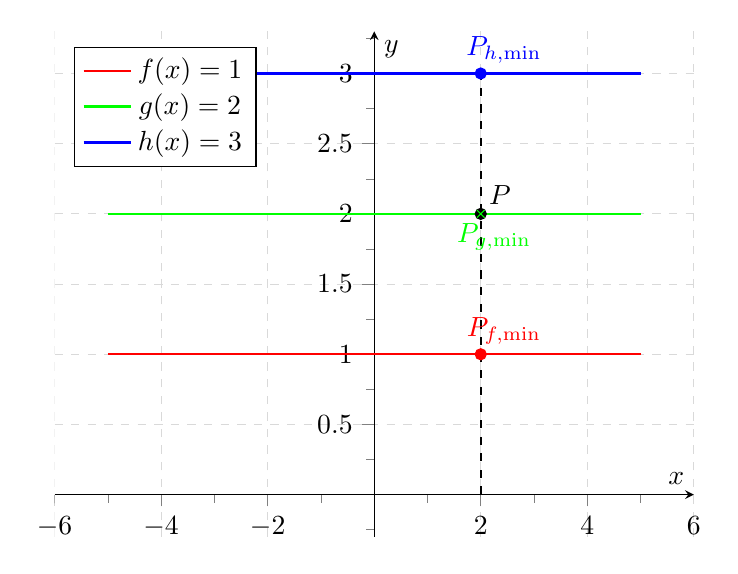
\begin{tikzpicture}
        \begin{axis}[
            legend pos=north west,
            axis x line=middle,
            axis y line=middle,
            grid = major,
            width=0.8\linewidth,
            height=8cm,
            grid style={dashed, gray!30},
            xmin=-5, % start the diagram at this x-coordinate
            xmax= 5, % end   the diagram at this x-coordinate
            ymin= 0, % start the diagram at this y-coordinate
            ymax= 3, % end   the diagram at this y-coordinate
            axis background/.style={fill=white},
            xlabel=$x$,
            ylabel=$y$,
            tick align=outside,
            minor tick num=-3,
            enlargelimits=true,
            tension=0.08]
          \addplot[domain=-5:5, thick,samples=50, red] {1};
          \addplot[domain=-5:5, thick,samples=50, green] {2};
          \addplot[domain=-5:5, thick,samples=50, blue] {3};
          \addplot[black, mark = *, nodes near coords=$P$,every node near coord/.style={anchor=225}] coordinates {(2, 2)};
          \addplot[blue, mark = *, nodes near coords=$P_{h,\text{min}}$,every node near coord/.style={anchor=225}] coordinates {(2, 3)};
          \addplot[green, mark = x, nodes near coords=$P_{g,\text{min}}$,every node near coord/.style={anchor=120}] coordinates {(2, 2)};
          \addplot[red, mark = *, nodes near coords=$P_{f,\text{min}}$,every node near coord/.style={anchor=225}] coordinates {(2, 1)};
          \draw[thick, dashed] (axis cs:2,0) -- (axis cs:2,3);
          \addlegendentry{$f(x)=1$}
          \addlegendentry{$g(x)=2$}
          \addlegendentry{$h(x)=3$}
        \end{axis} 
    \end{tikzpicture}
    \caption{Three constant functions and their points with minimal distance}
    \label{fig:constant-min-distance}
\end{figure}

Then $(x_P,f(x_P))$ has
minimal distance to $P$. Every other point has higher distance.
See Figure~\ref{fig:constant-min-distance}.

%%%%%%%%%%%%%%%%%%%%%%%%%%%%%%%%%%%%%%%%%%%%%%%%%%%%%%%%%%%%%%%%%%%%%
% Linear functions                                                  %
%%%%%%%%%%%%%%%%%%%%%%%%%%%%%%%%%%%%%%%%%%%%%%%%%%%%%%%%%%%%%%%%%%%%%
\section{Minimal distance to a linear function}
Let $f(x) = m \cdot x + t$ with $m \in \mdr \setminus \Set{0}$ and 
$t \in \mdr$ be a linear function.

\begin{figure}[htp]
    \centering
    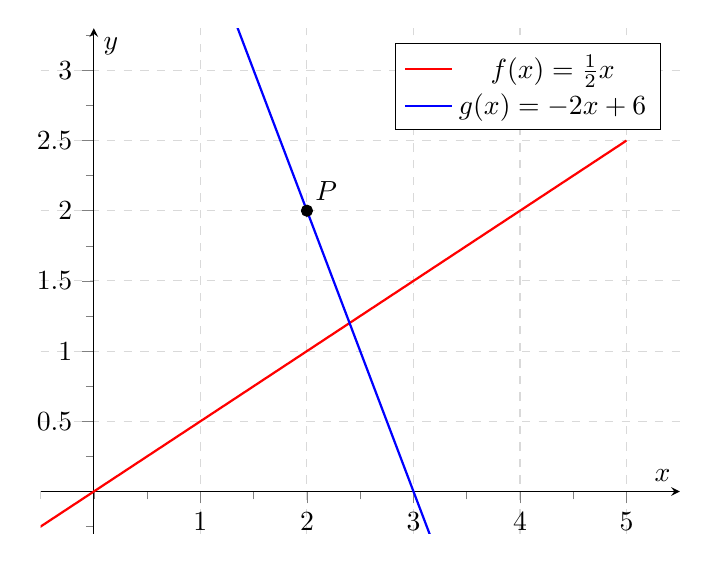
\begin{tikzpicture}
        \begin{axis}[
            legend pos=north east,
            axis x line=middle,
            axis y line=middle,
            grid = major,
            width=0.8\linewidth,
            height=8cm,
            grid style={dashed, gray!30},
            xmin= 0, % start the diagram at this x-coordinate
            xmax= 5, % end   the diagram at this x-coordinate
            ymin= 0, % start the diagram at this y-coordinate
            ymax= 3, % end   the diagram at this y-coordinate
            axis background/.style={fill=white},
            xlabel=$x$,
            ylabel=$y$,
            tick align=outside,
            minor tick num=-3,
            enlargelimits=true,
            tension=0.08]
          \addplot[domain=-5:5, thick,samples=50, red] {0.5*x};
          \addplot[domain=-5:5, thick,samples=50, blue] {-2*x+6};
          \addplot[black, mark = *, nodes near coords=$P$,every node near coord/.style={anchor=225}] coordinates {(2, 2)};
          \addlegendentry{$f(x)=\frac{1}{2}x$}
          \addlegendentry{$g(x)=-2x+6$}
        \end{axis} 
    \end{tikzpicture}
    \caption{The shortest distance of $P$ to $f$ can be calculated by using the perpendicular}
    \label{fig:linear-min-distance}
\end{figure}

Now you can drop a perpendicular $f_\bot$ through $P$ on $f(x)$. The slope of $f_\bot$
is $- \frac{1}{m}$. Now you can calculate $f_\bot$:\nobreak
\begin{align}
                 f_\bot(x) &= - \frac{1}{m} \cdot x + t_\bot\\
    \Rightarrow        y_P &= - \frac{1}{m} \cdot x_P + t_\bot\\
    \Leftrightarrow t_\bot &= y_P + \frac{1}{m} \cdot x_P
\end{align}

Now find the point $(x, f(x))$ where the perpendicular crosses the function:
\begin{align}
    f(x) &= f_\bot(x)\\
    \Leftrightarrow m \cdot x + t &= - \frac{1}{m} \cdot x + \left(y_P + \frac{1}{m} \cdot x_P \right)\\
    \Leftrightarrow \left (m + \frac{1}{m} \right ) \cdot x &= y_P + \frac{1}{m} \cdot x_P - t\\
    \Leftrightarrow x &= \frac{m}{m^2+1} \left ( y_P + \frac{1}{m} \cdot x_P - t \right )
\end{align}

There is only one point with minimal distance. See Figure~\ref{fig:linear-min-distance}.
\clearpage
%%%%%%%%%%%%%%%%%%%%%%%%%%%%%%%%%%%%%%%%%%%%%%%%%%%%%%%%%%%%%%%%%%%%%
% Quadratic functions                                               %
%%%%%%%%%%%%%%%%%%%%%%%%%%%%%%%%%%%%%%%%%%%%%%%%%%%%%%%%%%%%%%%%%%%%%
\section{Minimal distance to a quadratic function}
Let $f(x) = a \cdot x^2 + b \cdot x + c$ with $a \in \mdr \setminus \Set{0}$ and 
$b, c \in \mdr$ be a quadratic function.

\begin{figure}[htp]
    \centering
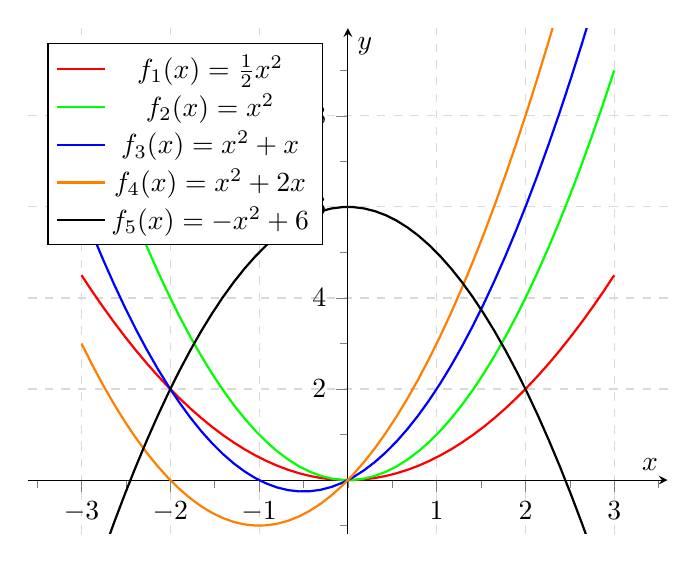
\begin{tikzpicture}
    \begin{axis}[
        legend pos=north west,
        axis x line=middle,
        axis y line=middle,
        grid = major,
        width=0.8\linewidth,
        height=8cm,
        grid style={dashed, gray!30},
        xmin=-3,     % start the diagram at this x-coordinate
        xmax= 3,    % end   the diagram at this x-coordinate
        ymin=-0.25,     % start the diagram at this y-coordinate
        ymax= 9,   % end   the diagram at this y-coordinate
        axis background/.style={fill=white},
        xlabel=$x$,
        ylabel=$y$,
        %xticklabels={-2,-1.6,...,7},
        %yticklabels={-8,-7,...,8},
        tick align=outside,
        minor tick num=-3,
        enlargelimits=true,
        tension=0.08]
      \addplot[domain=-3:3, thick,samples=50, red] {0.5*x*x}; 
      \addplot[domain=-3:3, thick,samples=50, green] {x*x}; 
      \addplot[domain=-3:3, thick,samples=50, blue] {x*x + x};
      \addplot[domain=-3:3, thick,samples=50, orange] {x*x + 2*x};
      \addplot[domain=-3:3, thick,samples=50, black] {-x*x + 6};
      \addlegendentry{$f_1(x)=\frac{1}{2}x^2$}
      \addlegendentry{$f_2(x)=x^2$}
      \addlegendentry{$f_3(x)=x^2+x$}
      \addlegendentry{$f_4(x)=x^2+2x$}
      \addlegendentry{$f_5(x)=-x^2+6$}
    \end{axis} 
\end{tikzpicture}
    \caption{Quadratic functions}
\end{figure}

\subsection{Calculate points with minimal distance}
In this case, $d_{P,f}^2$ is polynomial of degree 4. 
We use Theorem~\ref{thm:required-extremum-property}:\nobreak
\begin{align}
    0     &\overset{!}{=} (d_{P,f}^2)'\\
          &= -2 x_p + 2x -2y_p f'(x) + \left (f(x)^2 \right )'\\
          &= -2 x_p + 2x -2y_p f'(x) + 2 f(x) \cdot f'(x) \rlap{\hspace*{3em}(chain rule)}\label{eq:minimizingFirstDerivative}\\
\Leftrightarrow 0 &\overset{!}{=} -x_p + x -y_p f'(x) + f(x) \cdot f'(x) \rlap{\hspace*{3em}(divide by 2)}\label{eq:minimizingFirstDerivative}\\
          &= -x_p + x -y_p (2ax+b) + (ax^2+bx+c)(2ax+b)\\
          &= -x_p + x -y_p \cdot 2ax- y_p b + (2 a^2 x^3+2 a b x^2+2 a c x+ab x^2+b^2 x+bc)\\
          &= -x_p + x -2y_p ax- y_p b + (2a^2 x^3 + 3 ab x^2 + 2acx + b^2 x + bc)\\
          &= 2a^2 x^3 + 3 ab x^2 + (1 -2y_p a+ 2ac + b^2)x +(bc-by_p-x_p)\label{eq:quadratic-derivative-eq-0}
\end{align}

%\begin{align}
%    0     &\overset{!}{=}(d_{P,f}^2)''\\
%          &= 2 - 2y_p f''(x) + \left ( 2 f(x) \cdot f'(x) \right )' \rlap{\hspace*{3em}(Eq. \ref{eq:minimizingFirstDerivative})}\\
%          &= 2 - 2y_p f''(x) + 2 \cdot \left ( f'(x) \cdot f'(x) + f(x) \cdot f''(x) \right ) \rlap{\hspace*{3em}(product rule)}\\
%          &= 2 - 2y_p f''(x) + 2 \cdot \left ( f'(x)^2 + f(x) \cdot f''(x) \right )\\
%          &= 12a^2 x^2 + 12abx + 2(1 -2y_p a+ 2ac + b^2)
%\end{align}


This is an algebraic equation of degree 3.
There can be up to 3 solutions in such an equation. Those solutions
can be found with a closed formula.

\todo[inline]{Where are those closed formulas?}

\begin{example}
    Let $a = 1,  b = 0,  c= 1, x_p= 0, y_p = 1$.
    So $f(x) = x^2 + 1$ and $P(0, 1)$.

\begin{align}
    0 &\stackrel{!}{=} 4 x^3 - 2x\\
      &=2x(2x^2 - 1)\\
    \Rightarrow x_1 &= 0 \;\;\; x_{2,3} = \pm \frac{1}{\sqrt{2}}
\end{align}

As you can easily verify, only $x_1$ is a minimum of $d_{P,f}$.
\end{example}


\subsection{Number of points with minimal distance}
\subsubsection{Two points with minimal distance}
Quadratic functions can have two points with minimal distance. 

For example, let $f(x) = x^2$ and $P = (0,5)$. Then $P_{f,1} = (\sqrt{\frac{9}{2}}, \frac{9}{2})$
has minimal distance to $P$, but also $P_{f,2} = (-\sqrt{\frac{9}{2}}, \frac{9}{2})$:

\begin{proof}
    \begin{align}
      d_{P,f}(x)  &= \sqrt{(x-x_P)^2 + (f(x)-y_p)^2}\\
        &= \sqrt{x^2 + (x^2-5)^2}\\
        &= \sqrt{x^2 + x^4-10x^2+25}\\
        &= \sqrt{x^4 -9x^2 + 25}\\
        &= \sqrt{x^4 -9x^2 + \frac{81}{4}+\frac{19}{4}}\\
        &= \sqrt{\left (x^2 - \frac{9}{2} \right )^2 + \frac{19}{4}}
    \end{align}

    Obviously, $d_{P,f}$ is minimal for $x = \pm \sqrt{\frac{9}{2}} \qed$
\end{proof}

\begin{figure}[htp]
    \centering
    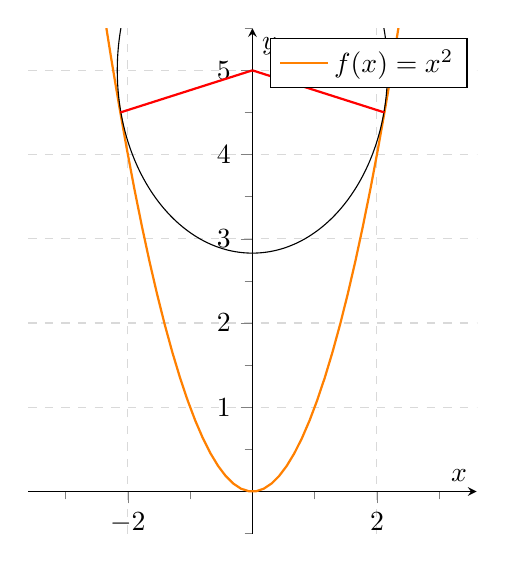
\begin{tikzpicture}
        \begin{axis}[
            %legend pos=north west,
            axis x line=middle,
            axis y line=middle,
            grid = major,
            width=0.6\linewidth,
            height=8cm,
            grid style={dashed, gray!30},
            xmin=-3,     % start the diagram at this x-coordinate
            xmax= 3,    % end   the diagram at this x-coordinate
            ymin= 0,     % start the diagram at this y-coordinate
            ymax= 5,   % end   the diagram at this y-coordinate
            axis background/.style={fill=white},
            xlabel=$x$,
            ylabel=$y$,
            %xticklabels={-2,-1.6,...,7},
            %yticklabels={-8,-7,...,8},
            tick align=outside,
            minor tick num=-3,
            enlargelimits=true,
            tension=0.08]
          \addplot[domain=-3:3, thick,samples=50, orange] {x*x};
          \draw (axis cs:0,5) circle[radius=2.17];
          \draw[red, thick] (axis cs:0,5) -- (axis cs:2.121,4.5);
          \draw[red, thick] (axis cs:0,5) -- (axis cs:-2.121,4.5);
          \addlegendentry{$f(x)=x^2$}
        \end{axis} 
    \end{tikzpicture}
    \caption{Two points with minimal distance}
\end{figure}

\subsubsection{Three points with minimal distance}
As discussed before, there cannot be more than 3 points on the graph
of $f$ next to $P$.

\todo[inline]{But can there be three points? O.b.d.A: $a > 0$.
As $c$ is moves the curve only up and down, we can o.b.d.A assume
that $c=0$. 

$x=-\frac{b}{2a}$ is the minimum of $f$. If there are 3 points, this will
be one of them. The other two ones are symmetric by an axis through
$-\frac{b}{2a}$}

\begin{figure}[htp]
    \centering
    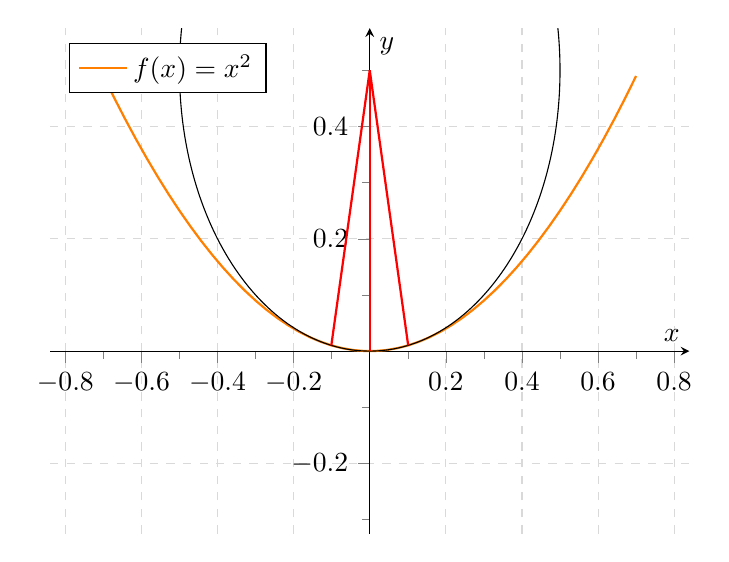
\begin{tikzpicture}
        \begin{axis}[
            legend pos=north west,
            axis x line=middle,
            axis y line=middle,
            grid = major,
            width=0.8\linewidth,
            height=8cm,
            grid style={dashed, gray!30},
            xmin=-0.7,     % start the diagram at this x-coordinate
            xmax= 0.7,    % end   the diagram at this x-coordinate
            ymin=-0.25,     % start the diagram at this y-coordinate
            ymax= 0.5,   % end   the diagram at this y-coordinate
            axis background/.style={fill=white},
            xlabel=$x$,
            ylabel=$y$,
            %xticklabels={-2,-1.6,...,7},
            %yticklabels={-8,-7,...,8},
            tick align=outside,
            minor tick num=-3,
            enlargelimits=true,
            tension=0.08]
          \addplot[domain=-0.7:0.7, thick,samples=50, orange] {x*x};
          \draw (axis cs:0,0.5) circle[radius=0.5];
          \draw[red, thick] (axis cs:0,0.5) -- (axis cs:0.101,0.0102);
          \draw[red, thick] (axis cs:0,0.5) -- (axis cs:-0.101,0.0102);
          \draw[red, thick] (axis cs:0,0.5) -- (axis cs:0,0);
          \addlegendentry{$f(x)=x^2$}
        \end{axis} 
    \end{tikzpicture}
    \caption{3 points with minimal distance?}
\end{figure}

When move the $f$ and $P$ simultaneously in $x$ direction, you will not change the
results. 

First of all, you move $f_0$ by $\frac{b}{2a}$, so
\[f_1(x) = ax^2 - \frac{b^2}{4a} + c \;\;\;\text{ and }\;\;\; P_1 = \left (x_p+\frac{b}{2a},\;\; y_p \right )\]

Because:
\begin{align}
    f(x-\nicefrac{b}{2a}) &= a (x-\nicefrac{b}{2a})^2 + b (x-\nicefrac{b}{2a}) + c\\
    &= a (x^2 - \nicefrac{b}{a} x + \nicefrac{b^2}{4a^2}) + bx - \nicefrac{b^2}{2a} + c\\
    &= ax^2 - bx + \nicefrac{b^2}{4a} + bx - \nicefrac{b^2}{2a} + c\\
    &= ax^2 -\nicefrac{b^2}{4a} + c
\end{align}


Then move $f_1$ and $P_1$ by $\frac{b^2}{4a}-c$ in $y$ direction. You get:
\[f_2(x) = ax^2\;\;\;\text{ and }\;\;\; P_2 = \left (x_p+\frac{b}{2a},\;\; y_p+\frac{b^2}{4a}-c \right )\]

As $f(x) = ax^2$ is symmetric to the $y$ axis, only points 
$P = (0, y_p)$ could possilby have three minima.

Then compute:
\begin{align}
  d_{P,f}(x)  &= \sqrt{(x-x_P)^2 + (f(x)-y_p)^2}\\
    &= \sqrt{x^2 + (ax^2-y_p)^2}\\
    &= \sqrt{x^2 + a^2 x^4-2ay_p x^2+y_p^2}\\
    &= \sqrt{a^2 x^4 + (1-2ay_p) x^2 + y_p^2}\\
    &= \sqrt{\left (a^2 x^2 + \frac{1-2 a y_p}{2} \right )^2 + y_p^2 - (1-2 a y_p)^2}\\
    &= \sqrt{\left (a^2 x^2 + \nicefrac{1}{2}-a y_p \right )^2 + (y_p^2 - (1-2 a y_p)^2)}\\
\end{align}

For $y_p \leq \nicefrac{1}{2a}$ you only have $x = 0$ as a minimum.
For all other points, there are exactly two minima.

\clearpage
%%%%%%%%%%%%%%%%%%%%%%%%%%%%%%%%%%%%%%%%%%%%%%%%%%%%%%%%%%%%%%%%%%%%%
% Cubic                                                             %
%%%%%%%%%%%%%%%%%%%%%%%%%%%%%%%%%%%%%%%%%%%%%%%%%%%%%%%%%%%%%%%%%%%%%
\section{Minimal distance to a cubic function}
Let $f(x) = a \cdot x^3 + b \cdot x^2 + c \cdot x + d$ be a cubic function
with $a \in \mdr \setminus \Set{0}$ and 
$b, c, d \in \mdr$ be a function.

\begin{figure}[htp]
    \centering
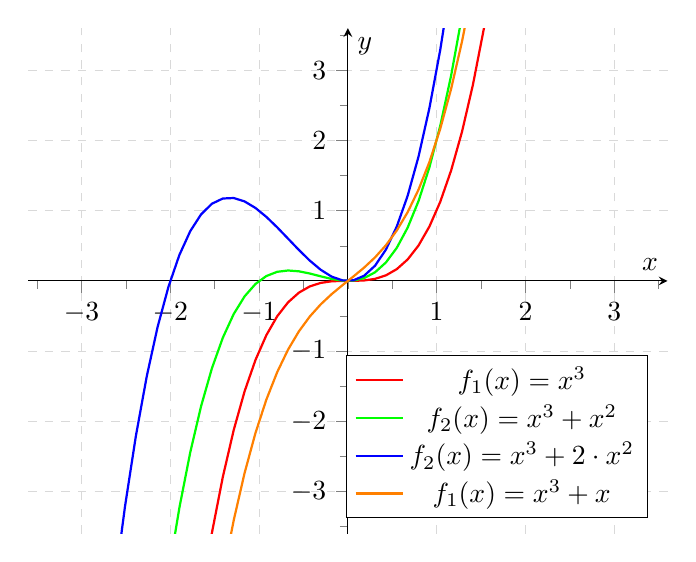
\begin{tikzpicture}
    \begin{axis}[
        legend pos=south east,
        axis x line=middle,
        axis y line=middle,
        grid = major,
        width=0.8\linewidth,
        height=8cm,
        grid style={dashed, gray!30},
        xmin=-3,     % start the diagram at this x-coordinate
        xmax= 3,    % end   the diagram at this x-coordinate
        ymin=-3,     % start the diagram at this y-coordinate
        ymax= 3,   % end   the diagram at this y-coordinate
        axis background/.style={fill=white},
        xlabel=$x$,
        ylabel=$y$,
        %xticklabels={-2,-1.6,...,7},
        %yticklabels={-8,-7,...,8},
        tick align=outside,
        minor tick num=-3,
        enlargelimits=true,
        tension=0.08]
      \addplot[domain=-3:3, thick,samples=50, red] {x*x*x}; 
      \addplot[domain=-3:3, thick,samples=50, green] {x*x*x+x*x};
      \addplot[domain=-3:3, thick,samples=50, blue] {x*x*x+2*x*x};
      \addplot[domain=-3:3, thick,samples=50, orange] {x*x*x+x}; 
      \addlegendentry{$f_1(x)=x^3$}
      \addlegendentry{$f_2(x)=x^3 + x^2$}
      \addlegendentry{$f_2(x)=x^3 + 2 \cdot x^2$}
      \addlegendentry{$f_1(x)=x^3 + x$}
    \end{axis} 
\end{tikzpicture}
    \caption{Cubic functions}
\end{figure}

%
%\subsection{Special points}
%\todo[inline]{Write this}
%
%\subsection{Voronoi}
%
%For $b^2 \geq 3ac$
%
%\todo[inline]{Write this}

\subsection{Calculate points with minimal distance}
When you want to calculate points with minimal distance, you can 
take the same approach as in Equation \ref{eq:minimizingFirstDerivative}:

\begin{align}
    0  &\stackrel{!}{=} -2 x_p + 2x -2y_p(f(x))' + (f(x)^2)'\\
       &= 2 f(x) \cdot f'(x) - 2 y_p f'(x) + 2x - 2 x_p\\
       &= f(x) \cdot f'(x) - y_p f'(x) + x - x_p\\
       &= \underbrace{f'(x) \cdot \left (f(x) - y_p \right )}_{\text{Polynomial of degree 5}} + x - x_p
\end{align}

General algebraic equations of degree 5 don't have a solution formula.\footnote{TODO: Quelle}
Although here seems to be more structure, the resulting algebraic
equation can be almost any polynomial of degree 5:\footnote{Thanks to Peter Košinár on \href{http://math.stackexchange.com/a/584814/6876}{math.stackexchange.com} for this one}

\begin{align}
    0  &\stackrel{!}{=} f'(x) \cdot \left (f(x) - y_p \right ) + (x - x_p)\\
    &= \underbrace{3 a^2}_{= \tilde{a}} x^5 + \underbrace{5ab}_{\tilde{b}}x^4 + \underbrace{2(2ac + b^2 )}_{=: \tilde{c}}x^3 &+& \underbrace{3(ad+bc-ay_p)}_{\tilde{d}} x^2 \\
    & &+& \underbrace{(2 b d+c^2+1-2 b y_p)}_{=: \tilde{e}}x+\underbrace{c d-c y_p-x_p}_{=: \tilde{f}}\\
    0 &\stackrel{!}{=} \tilde{a}x^5 + \tilde{b}x^4 + \tilde{c}x^3 + \tilde{d}x^2 + \tilde{e}x + \tilde{f}
\end{align}

\begin{enumerate}
    \item With $a$, we can get any value of $\tilde{a} \in \mdr \setminus \Set{0}$.
    \item With $b$, we can get any value of $\tilde{b} \in \mdr \setminus \Set{0}$.
    \item With $c$, we can get any value of $\tilde{c} \in \mdr$.
    \item With $d$, we can get any value of $\tilde{d} \in \mdr$.
    \item With $y_p$, we can get any value of $\tilde{e} \in \mdr$.
    \item With $x_p$, we can get any value of $\tilde{f} \in \mdr$.
\end{enumerate}

The first restriction only guaratees that we have a polynomial of 
degree 5. The second one is necessary, to get a high range of
$\tilde{e}$.

This means, that there is no solution formula for the problem of 
finding the closest points on a cubic function to a given point.

\subsection{Number of points with minimal distance}
As there is an algebraic equation of degree 5, there cannot be more
than 5 solutions.
\todo[inline]{Can there be 3, 4 or even 5 solutions? Examples!

After looking at function graphs of cubic functions, I'm pretty 
sure that there cannot be 4 or 5 solutions, no matter how you 
chose the cubic function $f$ and $P$.

I'm also pretty sure that there is no polynomial (no matter what degree)
that has more than 3 solutions.}

\todo[inline]{If there is no closed form solution, I want to 
describe a numerical solution. I guess Newtons method might be good.}
\end{document}
